\chapter{Introduction}

\section{Tractive System}
\begin{figure}[h]
    \centering
    \includegraphics[scale=0.07]{tractive_system}
    \caption{Chimera Evoluzione's tractive system with the battery pack below the two inverters that are connected to the motors.}
    \label{fig:tractive_system}
\end{figure}
Tractive system refers to all the high-voltage components of the car. It includes the battery pack, the inverters and the electric motors that drive the wheels of the car.
As with Chimera Evoluzione, Fenice is powered by two independent three-phase permanent-magnet motors that drive the rear axle. Each motor is controlled by a motor controller that converts the direct current from the battery into a three-phase alternating current for the motors. By varying the output frequency and current, the controllers can set the motor's speed and torque. Motors and controllers are water-cooled while the battery is air-cooled.

\section{Batteries}
A battery is an electrical energy storage system that relies on chemical reactions to generate a voltage difference. The main properties of a battery are: nominal voltage, internal resistance, energy capacity and maximum discharge rate.

The voltage of a battery is influenced by many factors including: state of charge, temperature and applied load. The open-circuit voltage (OCV) of a Lithium-Ion battery cell is 4.2V at 100\% state of charge and 3.0V at 0\%.
When a load is applied to a cell, the voltage drops according to Ohm's law: $V_{dropped} = R_{internal}*I_{load}$. The higher the current drawn, the higher the voltage drop. In high power applications, this phenomenon can significantly reduce the usable energy of the battery.

\subsection{Battery Pack}
A battery pack is a group of cells connected in series and parallel to increase the electrical characteristics of the pack. Arranging the cells in series means that the current will only travel down a single path, passing through every cell. In this case, the voltage of the pack is equaled to the sum of every series.

In a parallel arrangement, the current travels down multiple paths, splitting across more cells. This increases the maximum current output of the battery, but the potential across all cells is equalized.
\begin{figure}[h]
    \centering
    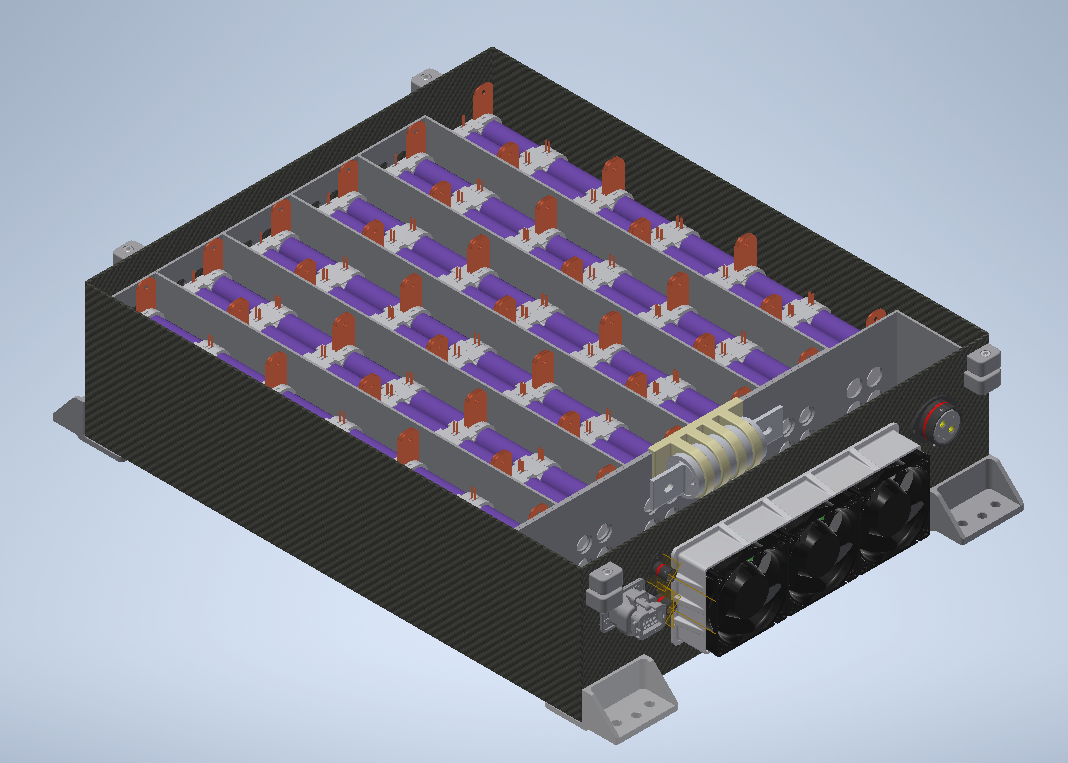
\includegraphics[scale=0.4]{pictures/pack.png}
    \caption{3D model of Fenice's battery pack}
    \label{fig:pack}
\end{figure}
The structure of a battery pack is decided considering its specific application. For example, in a high power context, higher voltage batteries are more desirable because for the same power draw, less current is required, reducing Joule effect heat losses across conductors. In high current applications, more cells in parallel could be arranged, increasing the total energy storage and battery weight as a consequence.

As mentioned above, a Formula SAE car's battery should be sized to complete a 22km endurance course while also being able to output the maximum amount of power for the acceleration event. The battery should also be optimized for weight and have a low center of gravity. Furthermore, the rulebook limits maximum voltage to 600V \cite[EV 4.1.1]{fsg2020} and power to 80kW \cite[EV 2.2.1]{fsg2020}, so the resulting battery will have as many cells in series as permitted and as few parallels as needed to reach the required power and capacity target.

Fenice's battery features 108 cells in series and 4 in parallel (108s4p), for a total of 432 cells and a nominal voltage of 388.8V. Higher voltages could be reached by rewiring the pack in a 144s3p configuration, but the pack would have a maximum voltage of 604.8V, exceeding the 600V limit. Adding more cells leads to increased weight, volume and excess capacity.

The high power requirement of the pack is fulfilled by the use of high-discharge rate cells, amounting to 45A in Fenice's case \cite{inr21700-40t}. This results in a total output of 180A of continuous discharge current. As a consequence, The maximum theoretical power output of the whole pack approaches 70kW and the energy capacity amounts to 6.2kWh.

\subsubsection{Naming hierarchy}
\begin{figure}[h]
    \centering
    \resizebox{\textwidth}{!}{%
        \begin{circuitikz}
    % Cell
    \draw (0,2) to[battery1] (0,3);
    \draw node[circle,draw,anchor=center,scale=4,label=Cell] (cell) at (0,2.5) {};

    % Cell to Module
    \draw node[circle,draw,anchor=center,scale=2.5] (ctm) at(2.25,2.5) {};
    \draw[->] (cell.east) -- (ctm.west);

    % Module
    \draw (2.75,1.5) -- ++(0,0.5) -| ++(-0.5,0) to[battery1] ++(0,1) -| ++(0.5,0.5)
    (2.75,2) -- ++(0.5,0) to[battery1] ++(0,1) -- ++(-0.5,0);
    \draw (3.25,2) edge[dotted] ++(0.5,0)
    (3.25,3) edge[dotted] ++(0.5,0);
    \draw node[circle,draw,anchor=center,scale=7,label=Module] (module) at (2.75,2.5) {};

    % Module to Block
    \draw node[circle,draw,anchor=center,scale=2.5] (mtb) at(6.5,2.5) {};
    \draw[->] (module.east) -- (mtb.west);

    % Block
    \draw (6.5,1) to[battery1] ++(0,1) to[battery1] ++(0,1) to[battery1] ++(0,1);
    \draw node[circle,draw,anchor=center,scale=9,label=Block] (block) at (6.5,2.5) {};

    % Block to Segment
    \draw[->] (block.east) -- (9.65,2.5);

    % Segment
    \draw (9.625,3) -- ++(0,+0.25);
    % 1
    \draw[solid] (9.5,2) rectangle ++(0.25,1);
    \draw (9.625,2) -- ++(0,-0.25) -| ++(0.5,0.25) ;
    % 2
    \draw[solid] (10,2) rectangle ++(0.25,1);
    \draw (10.125,3) -- ++(0,0.25) -| ++(0.5,-0.25) ;
    % 3
    \draw[solid] (10.5,2) rectangle ++(0.25,1);
    \draw (10.625,2) -- ++(0,-0.25) -| ++(0.5,0.25) ;
    % 4
    \draw[solid] (11,2) rectangle ++(0.25,1);
    \draw (11.125,3) -- ++(0,0.25) -| ++(0.5,-0.25) ;
    % 5
    \draw[solid] (11.5,2) rectangle ++(0.25,1);
    \draw (11.625,2) -- ++(0,-0.25) -| ++(0.5,0.25) ;
    % 6
    \draw[solid] (12,2) rectangle ++(0.25,1);
    \draw (12.125,3) -- ++(0,0.25);

    \draw node[circle,draw,anchor=center,scale=10,label=Segment] (segment) at (10.825,2.5) {};

    % Segment to Pack
    \draw[->] (segment.east) -- (14.15,2.5);

    % Pack
    \draw (14.125,3) -- ++(0,+0.25);
    % 1
    \draw[solid] (14,2) rectangle ++(0.25,1);
    \draw (14.125,2) -- ++(0,-0.25) -| ++(0.5,0.25) ;
    % 2
    \draw[solid] (14.5,2) rectangle ++(0.25,1);
    \draw (14.625,3) -- ++(0,0.25) -| ++(0.5,-0.25) ;
    % 3
    \draw[solid] (15,2) rectangle ++(0.25,1);
    \draw (15.125,2) -- ++(0,-0.25) -| ++(0.5,0.25) ;
    % 4
    \draw[solid] (15.5,2) rectangle ++(0.25,1);
    \draw (15.625,3) -- ++(0,0.25) -| ++(0.5,-0.25) ;
    % 5
    \draw[solid] (16,2) rectangle ++(0.25,1);
    \draw (16.125,2) -- ++(0,-0.25) -| ++(0.5,0.25) ;
    % 6
    \draw[solid] (16.5,2) rectangle ++(0.25,1);
    \draw (16.625,3) -- ++(0,0.25);

    \draw node[circle,draw,anchor=center,scale=10,label=Pack] (pack) at (15.4,2.5) {};

\end{circuitikz}%
    }
    \caption{Battery pack elements naming scheme}
    \label{fig:naming}
\end{figure}

As explained in \autoref{fig:naming}, the pack is subdivided into physical blocks that can be summarized as follows:

\begin{itemize}
    \item The \textbf{cell} is the basic unit of the pack.
    \item Four cells in parallel form a \textbf{module} (also called cell, since the voltage is the same as a single cell).
    \item \textbf{Blocks} are a series of three modules, held together to form an actual block.
    \item The rulebook requires the separation of the pack into \textbf{segments} with precise physical and electrical characteristics \cite[EV 5.3.2]{fsg2020}. In this case, a segment is a series of six blocks, totaling a maximum voltage of 75.6V ($4.2V*3\ modules*6\ blocks$) and 1.2kWh of energy, below the limit of 120V and 1.6 kWh mandated by the rules.
    \item In conclusion, the whole \textbf{pack} is composed of six segments connected in series.
\end{itemize}


\subsubsection{Battery insulation}
To be able to safely shut off the output of the battery pack, two normally-open Accumulator Isolation Relays (AIR) \cite[EV 5.6]{fsg2020} are located at both poles of the pack and can connect the internal battery terminals from the external connector located on the battery container.

The terminals of the battery pack must be always insulated from the rest of the low voltage system. For this reason, an insulation monitoring device (IMD) continuously checks for insulation between both the battery poles and the car's ground. The AIRs must disconnect if the insulation falls below a resistance greater than $\nicefrac{500\Omega}{V_{max}}$, where $V_{max}$ is the maximum pack voltage. The IMD is part of a broader circuit that drives the AIRs, called shutdown circuit.

\subsubsection{Shutdown Circuit}
The shutdown circuit carries the power that drives the coils of both AIRs. \autoref{fig:shutdown_circuit} shows the block schema of the circuit with all the safety switches and their normal state.
The most important switches are:
\begin{itemize}
    \item \textbf{LVMS} (Low-voltage master switch): Cuts low voltage power to the entire car. It is used as a power switch.
    \item \textbf{BSPD} (Brake switch plausibility device): a non-programmable circuit that opens when the brake and accelerator pedal are pressed simultaneously.
    \item \textbf{AMS} (Accumulator Management System): switch opened by the BMS in case of internal errors.
    \item \textbf{Shutdown Buttons}: Mushroom safety buttons located in the cockpit and on both sides of the car.
    \item \textbf{TSMS} (Tractive system master switch): similar to the LVMS, the TSMS is used to arm the tractive system before powering it on.
\end{itemize}

Being a critical and complex part of the car, problems with the shutdown circuit are common. In Chimera Evoluzione, there was no easy way of knowing the state of the shutdown circuit, so troubleshooting was hard and took considerable time. For Fenice, the circuit has been improved by adding 16 feedback connections to the BMS. Feedbacks are inputs on the microcontroller that are directly connected to various parts of the shutdown circuit to aid troubleshooting. Depending on its internal state, the BMS expects a certain set of feedbacks to be high and another set to be low; If some feedback signal is in an unexpected state, an error is triggered and the error management system takes over control.
\begin{figure}[h]
    \centering
    \begin{tikzpicture}
        \node(shutdown){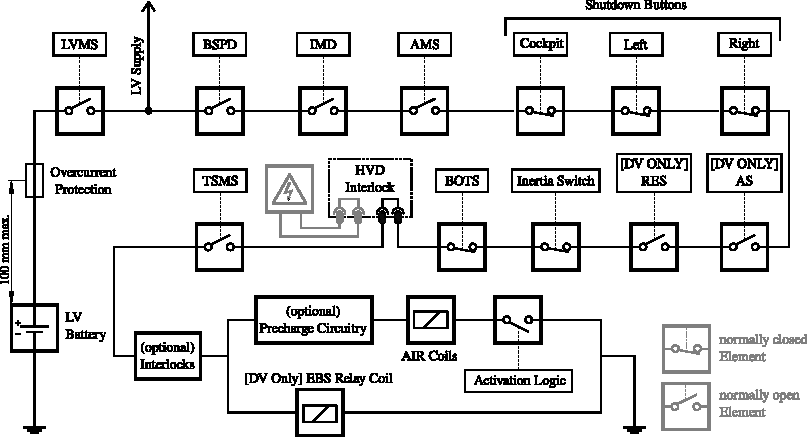
\includegraphics{pictures/shutdown_circuit}};
    \end{tikzpicture}
    \caption{Shutdown circuit block diagram \cite[EV 6.1.2]{fsg2020}}
    \label{fig:shutdown_circuit}
\end{figure}

For example: if the BMS is in the $Idle$ state, it expects the AIRs to be powered off. If the feedback for the AIR state is high an error is triggered, and if the problem persists for a set amount of time the pack goes into a critical error state.

\subsubsection{Pre-charge}
\begin{figure}[h]
    \centering
    \ctikzset{bipoles/crossing/size=.6}
\begin{circuitikz} \draw
    (0,1) to[battery=\(BAT\),american] ++(0,3)

    %% Negative battery bus
    (0,4) to[fuse=\(F\)] ++(1.5,0) to[nos=\(AIR-\), n=airm] ++(2,0) -- ++(1.5,0)
    -- (5, 2.6) to[short, -*] ++(2,0) -- (7, 4.5) -- ++(1.5,0)

    %% Inverter 1
    (7, 2.4) to[short, *-] (7.75,2.4) -- (7.75,3.5) -- (8.5,3.5)
    (8.5,3.5) to[C=\(C_1\), n=c1, *-*] (8.5,4.5)

    (8.5,0.5) -- ++(0.75,0)
    (8.5,1.5) -- ++(0.75,0);
    \draw[solid] (9.25,3.25) rectangle ++(0.5,1.5);
    \path (9.25,3.25) -- ++(0,-0.5);
    \draw[dotted] (7.3,5) rectangle (10,3) node[at start, right, fill=white] {Inverter 1};

    %% Positive battery bus
    \draw (0,1) to[nos=\(AIR+\), n=airp] ++(5,0)
    to (5,2.4) -- ++(2,0) -- (7, 0.5) -- ++(1.5,0)

    %% Inverter 2
    (7, 2.6) to[crossing] ++(1.5,0) -- (8.5,1.5)
    (8.5,0.5) to[C=\(C_2\), *-*] (8.5,1.5)

    (8.5,3.5) -- ++(0.75,0)
    (8.5,4.5) -- ++(0.75,0);
    \draw[solid] (9.25,1.75) rectangle ++(0.5,-1.5);
    \draw[dotted] (7.3,0) rectangle (10,2) node[at start, right, fill=white] {Inverter 2};

    %% Pre-charge circuit
    \draw (0.5,1) to[short, *-] ++(0,-1)
    to[nos=\(S_p\),n=pre_sw] ++(2, 0)
    to[R=\(R_p\),n=pre_sw] ++(2,0)
    to[short, -*] ++(0,+1)

    {[anchor=north] (6,2.4) node {\(Bus_+\)} [anchor=south] (6,2.6) node {\(Bus_-\)}};

    %% Motor 1
    \draw (11,4) node[elmech](M1){M1}
    (9.75,4.65) -- ++(0.75,0) -- (M1.150)
    (9.75,4) -| (M1.180)
    (9.75,3.35) -- ++(0.75,0) -- (M1.210)
    ;

    %% Motor 2
    \draw (11,1) node[elmech](M2){M2}
    (9.75,1.65) -- ++(0.75,0) -/ (M2.150)
    (9.75,1) -| (M2.180)
    (9.75,0.35) -- ++(0.75,0) -/ (M2.210)
    ;

    \draw[dotted] (-2,5) rectangle (5.25,-0.5) node[at start, right, fill=white] {Battery Pack};


\end{circuitikz}
    \caption{Tractive system schema highlighting the pre-charge circuitry}
    \label{fig:tractive_system_detail}
\end{figure}
If the power-on procedure of the pack simply involved putting both AIRs to their closed position, a potentially dangerous in-rush current would charge the capacitors on the inverters very quickly. To prevent over-current, the pre-charge procedure is performed \cite{precharge}. \autoref{fig:tractive_system_detail} shows the components of the pre-charge circuit.

First, the negative AIR and $S_p$ are closed. The resulting circuit has $R_p$ as the current-limiting resistor. After $Bus$ and $BAT$ voltages have equalized, the BMS commands the positive AIR to close. This completes the pre-charge procedure and the battery is now ready to be used.

\subsection{Battery Management System}
Battery management is a collection of operations that ensure the safety and efficiency of the battery pack. A basic battery management system should constantly measure cell temperatures and voltages along with the total pack current output and check that each of those values is within specification. If anomalies are detected, the battery should be disconnected immediately via the AIRs.
%\begin{figure}[h]
%    \centering
%    \begin{tikzpicture}[->, >=stealth', shorten >= 5pt, node  distance = 2.5cm, semithick]
        \node[state, initial]   (init)                                          {$Init$};
        \node[state]            (ts_off)    [right=of init]                     {$TS_{off}$};
        \node[state]            (idle)      [below left=2cm of ts_off]          {$Idle$};
        \node[state]            (pc_start)  [below=2cm of idle]                 {$PC_s$};
        \node[state]            (pc_wait)   [right=1.5cm of pc_start]           {$PC_w$};
        \node[state]            (pc_end)    [right=1.5cm of pc_wait]            {$PC_e$};
        \node[state]            (ts_on)     [above left=2cm and 1cm of pc_end]  {$TS_{on}$};
        \node[state]            (charge)    [above right=2cm and 1cm of pc_end] {$Chg$};
        \node[state]            (stacca)    [right=1.5cm of charge]             {$Stacca$};
        \node[state, accepting] (halt)      [below=1cm of stacca]               {$Halt$};
        \node[state]            (all)       [above=1cm of stacca]               {$*$};
        
        \path (init)        edge (ts_off);
        \path (ts_off)      edge[bend right=10] (idle);
        \path (idle)        edge[loop left] (idle)
                            edge (pc_start);
        \path (pc_start)    edge (pc_wait);
        \path (pc_wait)     edge[loop below] (pc_wait)
                            edge[bend left=5] (ts_off)
                            edge (pc_end);
        \path (pc_end)      edge[bend left=10] (ts_on)
                            edge[bend right=10] (charge);
        \path (ts_on)       edge[loop right] (ts_on)
                            edge[bend right=7] (ts_off);
        \path (charge)      edge[loop left] (charge)
                            edge[bend right] (ts_off);
        \path (stacca)      edge (halt);
        \path (halt)        edge[loop left] (halt);
        \path (all)         edge (stacca);
\end{tikzpicture}

%    \caption{Main BMS state machine}
%    \label{fig:fsm}
%\end{figure}

More advanced BMS implementations communicate their state of operation with other devices and turn the battery on or off according to external and internal signals.

Moreover, during battery charging, the BMS should handle the charge current curve to maximize charging speed while keeping the battery in a safe state. Cell balancing is also an important feature.

As the consequences of software errors on the BMS are potentially catastrophic, the code must adhere to strict standards and should be tested thoroughly. Furthermore, reliable error management should be present to abide by the rulebook and ease troubleshooting.

\subsubsection{Hardware}
The need to measure a large number of voltages and temperatures scattered around the battery pack leads to a decentralized structure for the BMS components. Two types of logic boards are involved, namely the \textbf{Mainboard} and the \textbf{Cellboard}.

\begin{figure}[h]
    \centering
    
\begin{tikzpicture}[
        text=blue,
        carnode/.style={inner sep=-11pt},
        mainnode/.style={rectangle, draw=red, fill=red!15, very thick, minimum size=10mm},
        cellnode/.style={rectangle, draw=yellow, fill=yellow!15, very thick},
        arrow/.style={<->, >=stealth, fill=white, draw=blue, very thick}
    ]


    %Nodes
    \node[carnode]  (car)                       {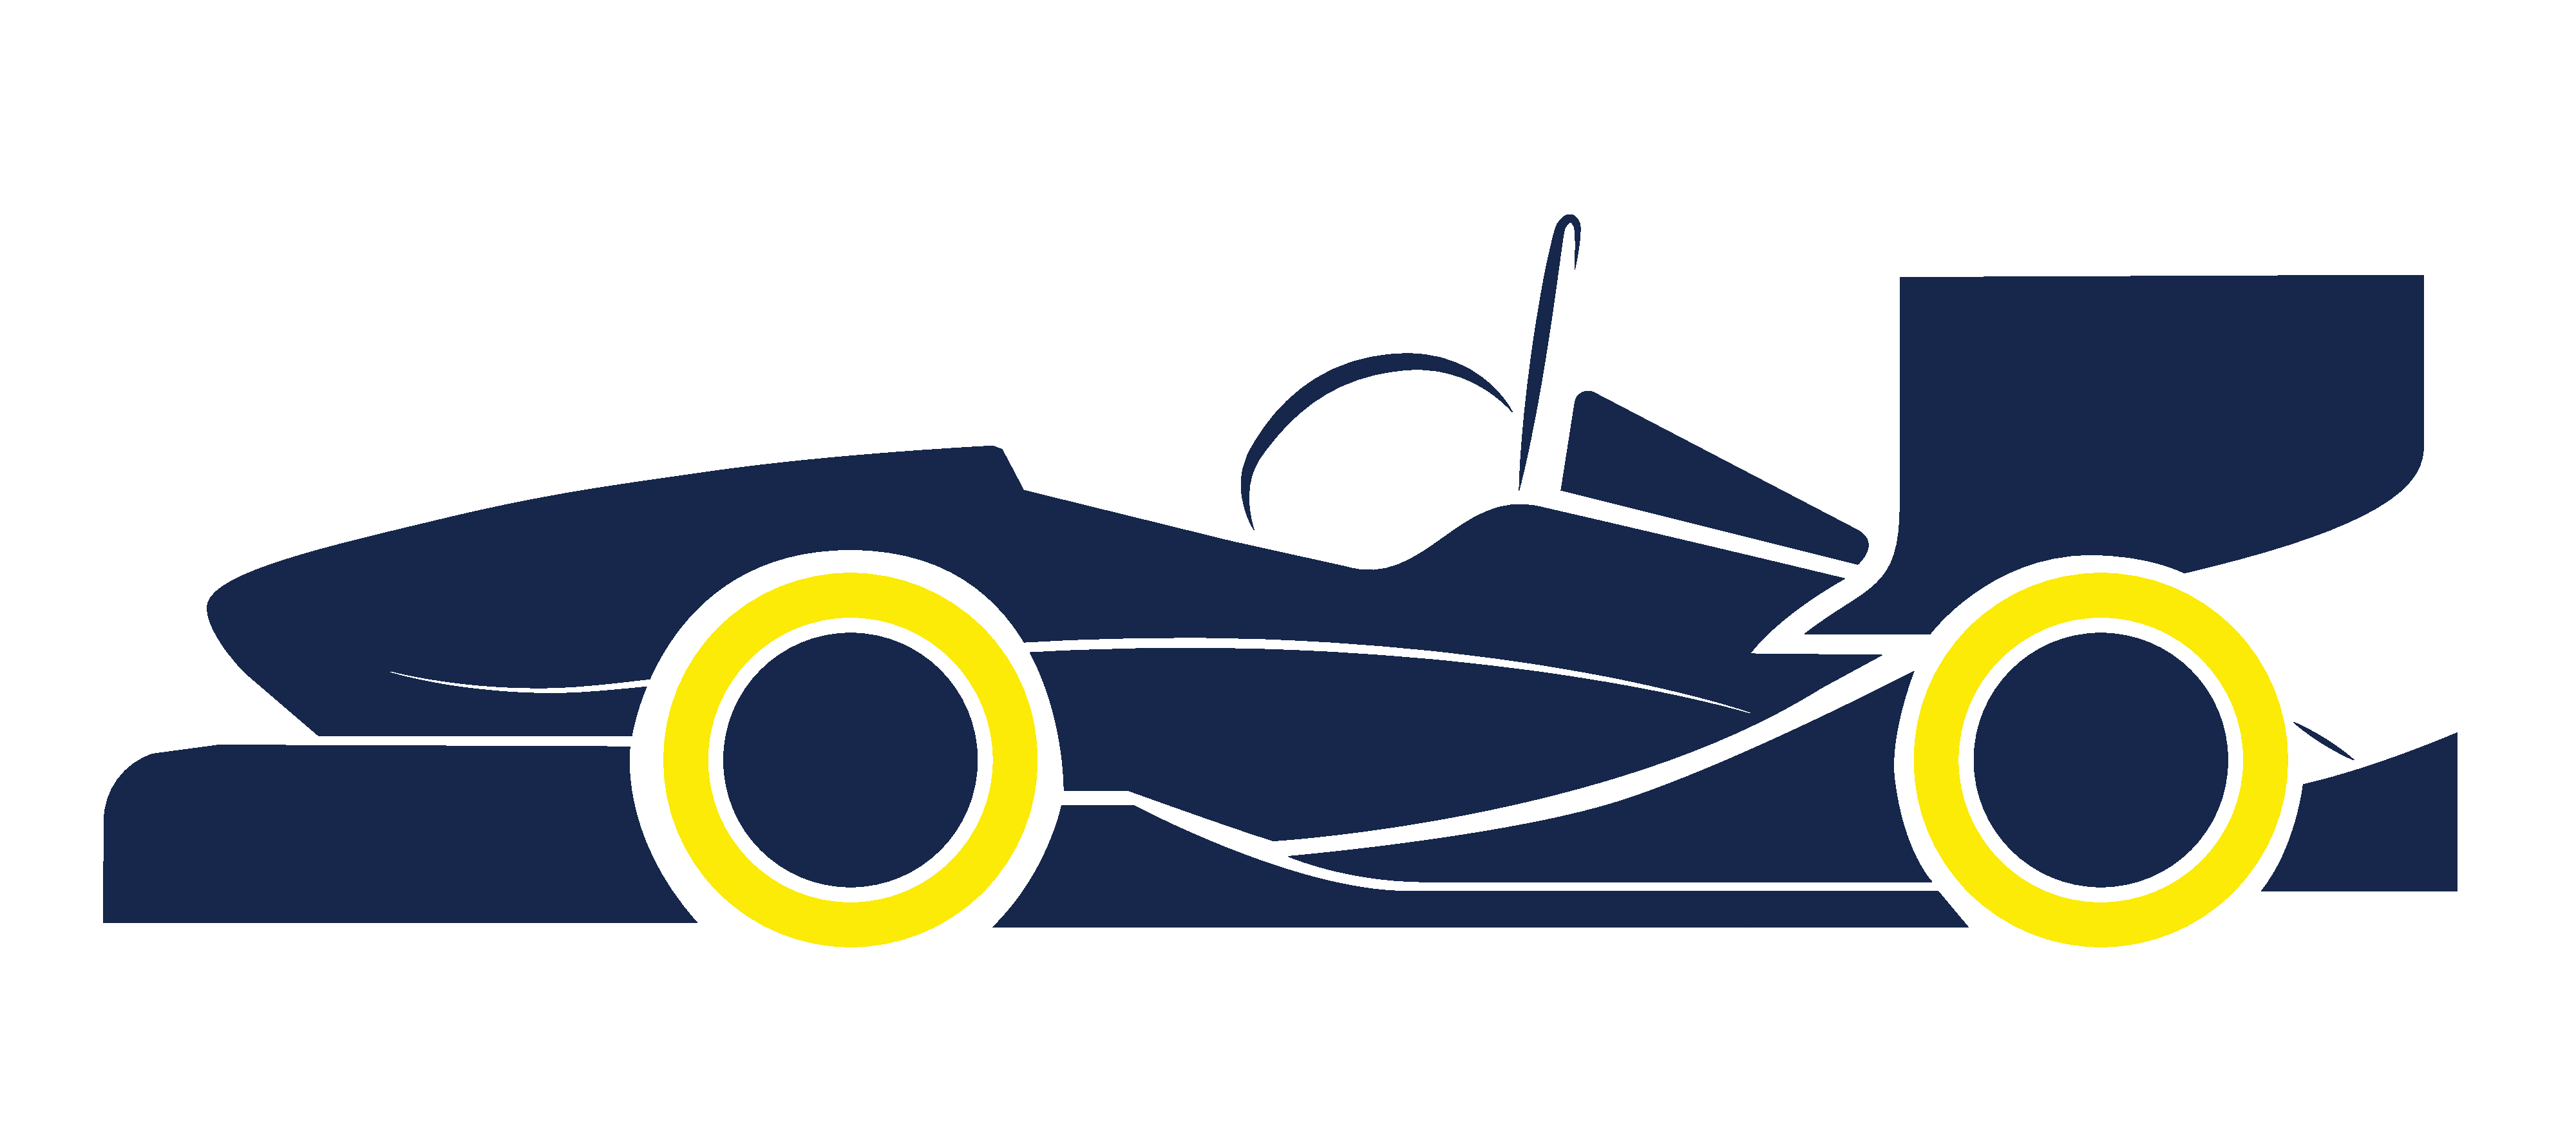
\includegraphics[width=0.3\textwidth, page=1]{silhouette.pdf}};
    \node[mainnode] (main)  [right=2cm of car]  {Mainboard};
    \node[cellnode] (c3)    [right=of main]     {Cellboard 3};
    \node[cellnode] (c2)    [right=of c3]       {Cellboard 2};
    \node[cellnode] (c1)    [above=of c2]       {Cellboard 1};
    \node[cellnode] (c0)    [left=of c1]        {Cellboard 0};
    \node[cellnode] (c4)    [below=of c3]       {Cellboard 4};
    \node[cellnode] (c5)    [right=of c4]       {Cellboard 5};

    %Lines
    \path [arrow] (main.north) node[anchor=south east] {\scriptsize{$master$}} |- node[above, fill=white] {CAN-bus} (c0.west);
    \path [arrow] (car.south) |- ++(0,-1) -- ++(2,0) node[fill=white] {CAN-bus} -| (main.south);

    \draw[arrow] (c0.east) -- (c1.west);
    \draw[arrow] (c1.south) -- (c2.north);
    \draw[arrow] (c2.west) -- (c3.east);
    \draw[arrow] (c3.south) -- (c4.north);
    \draw[arrow] (c4.east) -- (c5.west);

    %\draw let \p1=(main) \p2=(c0) in node at (\x1,\y2) {k};
    \draw[thick,dotted] ($(main.north west)+(-0.5, 2)$) rectangle ($(c5.south east)+(0.5, -0.5)$) node[at start, right, fill=white] {Battery};

\end{tikzpicture}

    \caption{BMS hierarchy}
    \label{fig:bms_hierarchy}
\end{figure}

\subsubsection{Mainboard}
%\begin{figure}[h]
%    \centering
%    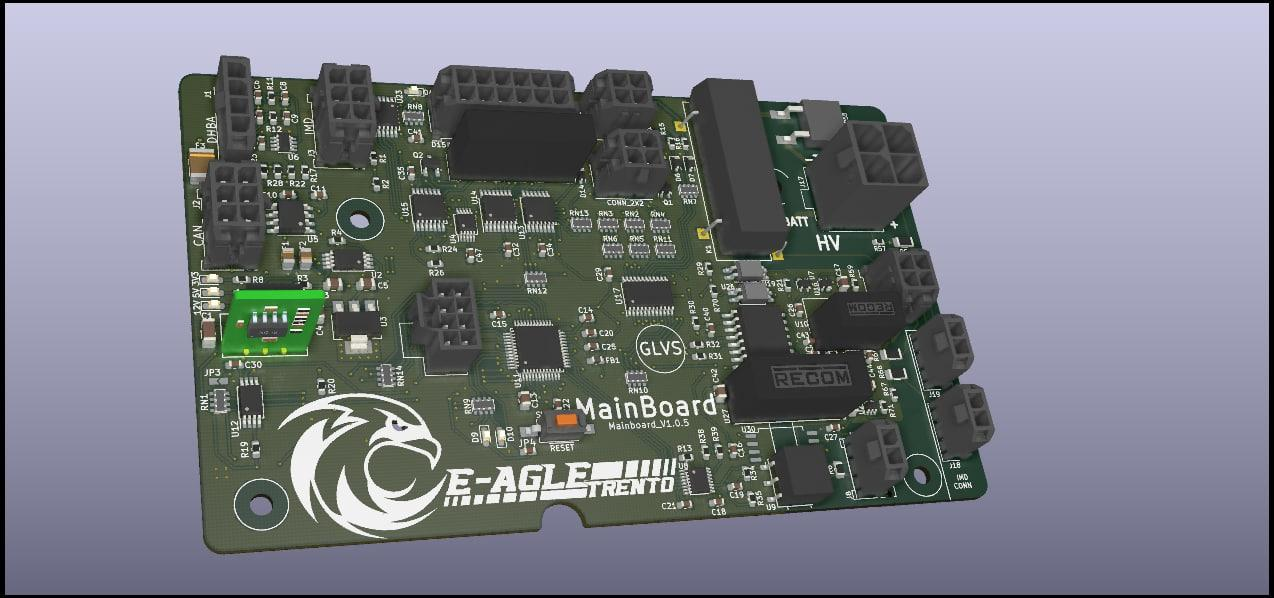
\includegraphics[scale=0.5]{pictures/mainboard.jpg}
%    \caption{Mainboard PCB}
%    \label{fig:mainboard}
%\end{figure}
The Mainboard is the central control unit of the BMS. It contains a microcontroller that handles two CAN-bus lines for internal and external communications, peripherals such as insulated ADCs, EEPROMs, serial ports, an SD-card and more. The mainboard is responsible for the actuation of the AIRs and contains the shutdown and pre-charge circuits. It also communicates voltages, temperatures, currents, battery status, warnings and errors to the rest of the car via CAN-bus. An integrated serial command-line interface and internal logging are included to help with troubleshooting.

\subsubsection{Cellboard}
Cellboards are dedicated to the measurement of module voltages and cell temperatures. The reading of voltages is handled by a specialized battery management chip that communicates via SPI to the onboard microcontroller. Temperatures are acquired with sensors glued to the busbars and are processed on board. All the data collected from the boards are sent via an internal CAN-bus to the mainboard.

Cellboards are also in control of cell balancing. They can activate and deactivate discharging for any module through the battery management chip, depending on commands from the mainboard and internal states.

The rulebook mandates that cellboards must be isolated from the mainboard; For this reason, the cellboards are self-powered by stepping down the battery segment's voltage. The communication is carried out with an isolated CAN-bus transceiver. Power for the insulated side of the transceiver coming from the mainboard also provides a power-on signal to the supply of the cellboard. In this way, if the mainboard is not powered, the cellboards don't draw current from the battery pack.

There are a total of six cellboards on Fenice's battery pack, one for every battery segment.

\section{Issues and objectives}
\subsection{Battery Management}

Work began by analyzing Chimera Evoluzione's BMS software, which ran on a slightly different architecture. While the software was functioning, it did not follow a consistent and modular structure and thus was not easily maintainable. A complete rewrite gives the possibility of implementing a more advanced and robust software architecture that is more maintainable and supports future improvements and additions while providing a better separation of features.

\subsection{Module Balancing}
Cells are not perfectly identical and can have slight variations in internal resistance between each other. These differences mean that after some use, modules can start to deviate in voltage between one another \cite{6966514}. If a cell has a higher voltage than average, the pack can only be charged to the voltage of said cell, while the remaining modules don't get fully charged. The same applies during discharge: if a module is more discharged than others, it constraints the maximum depth of discharge to when it reaches its cutoff voltage, while other cells are still above it and could theoretically be discharged further.

Chimera Evoluzione did not have the hardware required to mitigate the issue. This meant that cell voltages were slowly diverging, lowering usable capacity and affecting range. Cell balancing hardware is present on Fenice's BMS with some slight limitations.

The objective is to achieve the best cell balancing performance the hardware can offer.

\subsection{Error Management}
Error management is one of the more important features of a BMS. In Chimera Evoluzione errors were handled by hand with custom logic for every error type. Moreover, errors were only reported through the CAN network but were not logged internally or communicated through serial to a debugging computer. All these factors made on-track troubleshooting cumbersome and slow. Debugging issues were common amongst enclosed microcontrollers in Chimera Evoluzione. For this reason, significant effort was made towards the implementation of  efficient and effective error management and communication system. A centralized framework should handle all error types without distinction and logging should be integrated as well as CAN communication. The framework should be testable with offline unit tests to validate performance and stability. With this solid base, the management system can then be used to log a large variety of errors, ranging from safety-critical errors to minor issues with peripherals, enhancing online and offline troubleshooting for every situation.

\newpage

